\documentclass[12pt]{article}
\usepackage[english]{babel}
\usepackage{natbib}
\usepackage{url}
\usepackage{amsmath}
\usepackage{graphicx}
\graphicspath{{images/}}
\usepackage{parskip}
\usepackage{fancyhdr}
\usepackage{vmargin}
\usepackage{float}
\setmarginsrb{3 cm}{2.5 cm}{3 cm}{2.5 cm}{1 cm}{1.5 cm}{1 cm}{1.5 cm}

\title{The Library supports running deep learning on Intel Xeon Phi}                             % Title
\author{
  Nguyen Minh Tri\\
  Pham Duc Minh Chau\\
  Le Huynh Duy Thai\\
 }
\date{\today}                                           % Date

\makeatletter
\let\thetitle\@title
\let\theauthor\@author
\let\thedate\@date
\makeatother

\pagestyle{fancy}
\fancyhf{}
\lhead{\thetitle}
\cfoot{\thepage}

\begin{document}
%%%%%%%%%%%%%%%%%%%%%%%%%%%%%%%%%%%%%%%%%%%%%%%%%%%%%%%%%%%%%%%%%%%%%%%%%%%%%%%%%%%%%%%%%

\begin{titlepage}
    \centering
    \vspace*{0.5 cm}
    
\includegraphics[scale = 0.5]{hcmut.png}\\[1.0 cm]   % University Logo
    \textsc{\Large Ho Chi Minh City University of Technology}\\[1.0 cm]   % University Name
    \textsc{\Large Advanced Programming}\\[0.5 cm]               % Course Code
    \textsc{\large Assignment 2}\\[0.5 cm]               % Course Name
    \rule{\linewidth}{0.2 mm} \\[0.4 cm]
    { \LARGE \bfseries \thetitle}\\
    \rule{\linewidth}{0.2 mm} \\[1.5 cm]
    
    \begin{minipage}{0.4\textwidth}
        \begin{flushleft} \large
            \emph{Member:}\\
            \theauthor
            \end{flushleft}
            \end{minipage}~
            \begin{minipage}{0.4\textwidth}
            \begin{flushright} \large
            \emph{Student ID:} \\
            1770026 \\
            1770316\\
            1770320\\                                  % Your Student Number
        \end{flushright}
    \end{minipage}\\[2 cm]
    
    {\large \thedate}\\[2 cm]
 
    \vfill
    
\end{titlepage}

%%%%%%%%%%%%%%%%%%%%%%%%%%%%%%%%%%%%%%%%%%%%%%%%%%%%%%%%%%%%%%%%%%%%%%%%%%%%%%%%%%%%%%%%%

\renewcommand{\contentsname}{Contents}
\tableofcontents
\pagebreak

%%%%%%%%%%%%%%%%%%%%%%%%%%%%%%%%%%%%%%%%%%%%%%%%%%%%%%%%%%%%%%%%%%%%%%%%%%%%%%%%%%%%%%%%%

\section{Introduce}
Deep learning plays a vital role in broad spectrum of scientific fields, such as computer vision, speech recognition, natural language processing, and so on. In order to support deep learning, many frameworks are created with the aim of setting up artificial neural networks as quickly as possible. Such frameworks can be run on systems including either Graphical Processing Unit or Intel Xeon Phi the second generation Knights Landing coprocessor. However, very few deep learning frameworks can be run on legacy systems containing Intel Xeon Phi Knights Corner. For that reason, we propose and develop pyMIC$-$DL which is a NumPy$-$like library supporting deep learning frameworks run on such legacy systems.

\newpage

\section{Intel Xeon Phi}
\subsection{Introduction}

\begin{itemize}
\item Intel Xeon Phi coprocessors have been designed by Intel Corporation as supplement to the Intel Xeon processor family. The coprocessors feature the Intel manycore architecture, which enables fast and energy efficient execution of some High Performance Computing(HPC) applications. In most Intel communications, the term ``manycore", refers to the architecture of the Intel Xeon Phi product family, while ``multicore" architecture refers to the Intel Xeon family processors.

\begin{figure}[ht] 
  \begin{minipage}[b]{0.5\linewidth}
    \centering
      {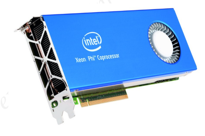
\includegraphics[width=0.95\linewidth]{chainer2.png}}
   	\caption{Manycore Intel Xeon Phi}
  \end{minipage}%%
  \begin{minipage}[b]{0.5\linewidth}
    \centering
      {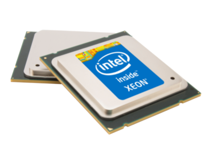
\includegraphics[width=0.95\linewidth]{chainer1.png}} 
    \caption{Multicore Intel Xeon}
  \end{minipage}
\end{figure}
\item The manycore architecture may yield more performance per watt of power and per dollar of setup costs than traditional multi-core CPUs. However, not every application can be accelerated by manycore coprocessors. Intel Xeon Phi coprocessors derive their high performance from multiple cores, dedicated vector arithmetic units with wide vector registers, and cached on board GDDR5. High energy efficiency is achieved using low clock speed x86 cores with lightweight design suitable for parallel HPC applications. Therefore, only highly parallel applications supporting vectorized arithmetic with well-behaved (or negligible) memory traffic will thrive on the manycore architecture.
\end{itemize}
\newpage
\subsection{Heterogeneous Computing and Clustering}
Programming models for Intel Xeon Phi coprocessors include native execution and offload-based approaches. These approaches enable developers to design a spectrum of hybrid computing models, ranging from multi-core hosted to multi-core-centric to symmetric and manycore-hosted. The choice of work division between the host and the coprocessor is dictated by the nature of the application. Highly parallel, vectorized workloads can be executed on the co-processor as well as on the host. However, serial segments of an application perform significantly better on Intel Xeon processors, and so do applications with stochastic memory access patterns. The overhead of data transport over the PCIe bus should also be taken into consideration. 
\begin{figure}[H]
\centering
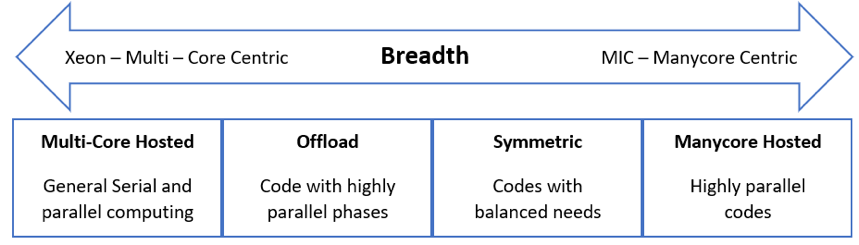
\includegraphics[scale = 0.9]{chainer3.png}
\caption{Programming model spectrum}
\end{figure}
\section{Native model}
Intel Xeon Phi coprocessors run a Linux operating system, with a virtual file system, a multi-user environment, and support for traditional Linux services, including SSH and NFS. These services allow the programmer to run applications directly on an Intel Xeon Phi coprocessor, without the involvement of the host. This does not mean that an application compiled for an Intel Xeon CPU will run on an Intel Xeon Phi coprocessor. Rather, it means that it is possible to compile an application for an Intel Xeon Phi coprocessor from the same source code as the CPU application. Then the executable and its dependent libraries must be transferred to, or shared with, the coprocessor's file system.

To compile a C, C++ code as an executable for the Intel Xeon Phi architecture, Intel compilers must be invoked with the argument -mmic.
\begin{figure}[H]
\centering
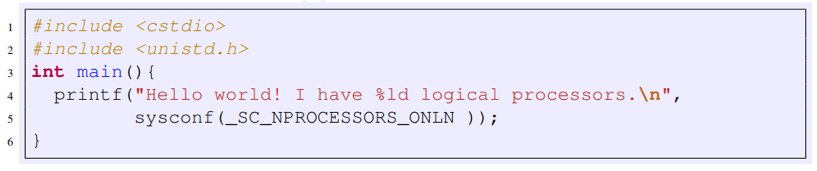
\includegraphics[scale = 0.9]{chainer4.png}
\caption{This C++ language code (``Native-Hello.cc") can be compiled for execution on the host as well as on an Intel Xeon Phi coprocessor.}
\end{figure}
\begin{figure}[H]
\centering
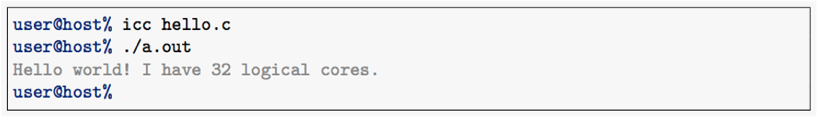
\includegraphics[scale = 0.9]{chainer5.png}
\caption{Compiling and running the ``Hello World" code on the host.}
\end{figure}

We can transfer the executable a.out to the coprocessor and use the shell to run the application on the coprocessor. Running this executable produces the expected ``Hello world" output, and the number of logical processors is correctly detected as 240.

\begin{figure}[H]
\centering
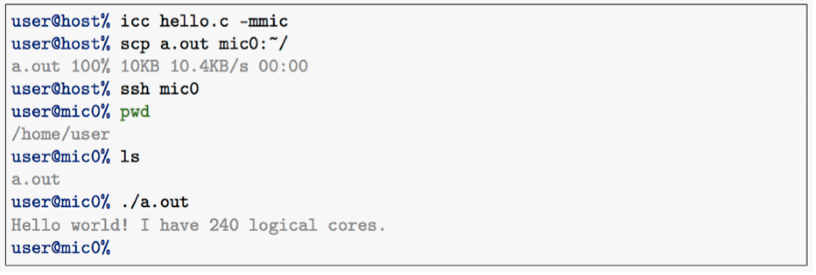
\includegraphics[scale = 0.9]{chainer6.png}
\caption{Transferring and running a native application on an Intel Xeon Phi coprocessor.}
\end{figure}
\newpage

\section{Offload programing model}
An alternative method is the so-called ``offload approach", where an application begins execution on the host, and at some point it employs the MIC architecture by transferring only some of the data and functions to run on the coprocessor. This process of data and code transfer to the coprocessor is generally called offload, and applications using this procedure are known as offload applications.
\begin{itemize}
\item ``HelloWorld" in Offload Model
\begin{figure}[H]
\centering
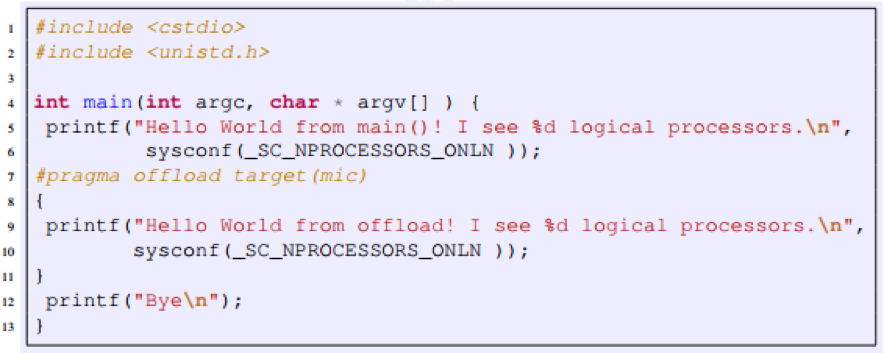
\includegraphics[scale = 0.9]{chainer7.png}
\caption{``Hello World" in the explicit offload model.}
\end{figure}
\end{itemize}

This application must be compiled as a usual host application:  no additional compiler arguments are necessary in order to compile offload applications. This code produces the following output:
\begin{figure}[H]
\centering
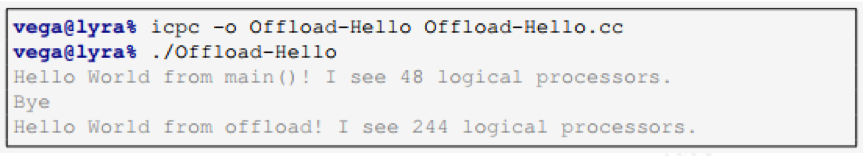
\includegraphics[scale = 0.9]{chainer8.png}
\caption{Output of the execution of Offload-Hello.cc.}
\end{figure}
In this context, it is worth mentioning that it is somewhat surprising that the line ``Bye" is the second printed line at runtime, even though in the original code it is the third line. At the same time, it should be surprising to the beginner reader that``Hello from offload" was printed at all, because it was output into stdout of the OS. The output to the coprocessor's stdout is buffered and mirrored in the host console, and the consistency of the order of output is therefore not guaranteed.

In this example, initiating offload with \#pragma offload is trivial, because all code and all data in the offload region exist only in the scope of \#pragma offload. However, when functions or data need to be offloaded, offload programming will require more customization of the offload directive.

\subsection{Offloading Functions}
When user defined functions are called in an offload region, they must be declared with the qualifier $\_\_attribute\_\_ ((target(mic)))$ . This qualifier tells the compiler to generate the MIC architecture executable code for the function.
\begin{figure}[H]
\centering
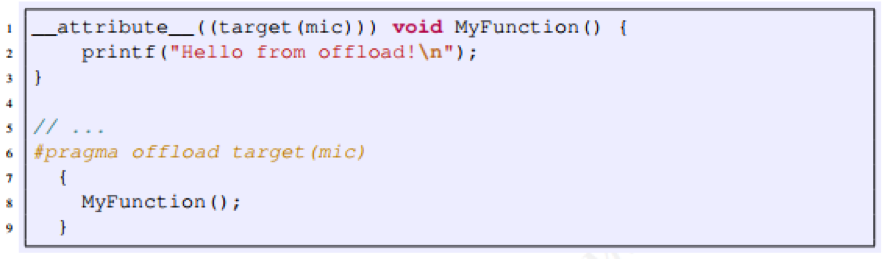
\includegraphics[scale = 0.9]{chainer9.png}
\caption{Offloading a function to an Intel Xeon Phi coprocessor.}
\end{figure}

If multiple functions must be declared with this qualifier, there is a shorthand way to set and unset this qualifier inside a source file: use \#pragma offload attribute(push/pop).
\begin{figure}[H]
\centering
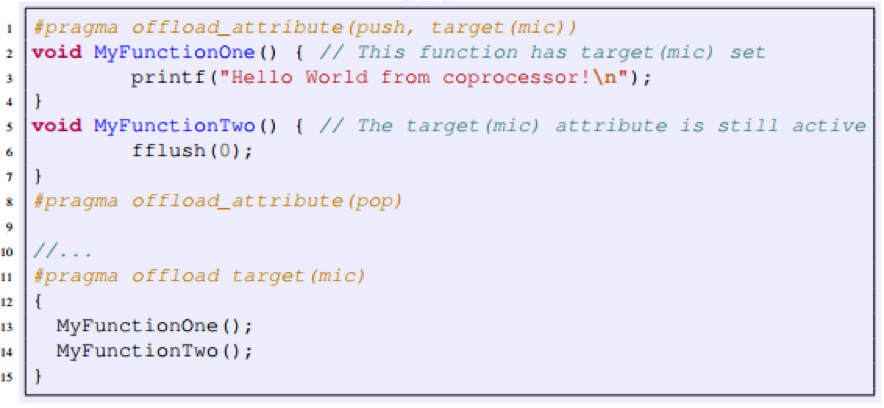
\includegraphics[scale = 0.9]{chainer10.png}
\caption{Declaring multiple functions with the target attribute qualifier.}
\end{figure}
\subsection{Offloading Scope-Local Data}
Local scalar variables and arrays of known size are automatically transferred to and from the coprocessor at the start and the end of the offload, respectively. However this behavior can be modified by including them into one of the clauses of the offload pragma: $in, out, inout, nocopy$.
\begin{figure}[H]
\centering
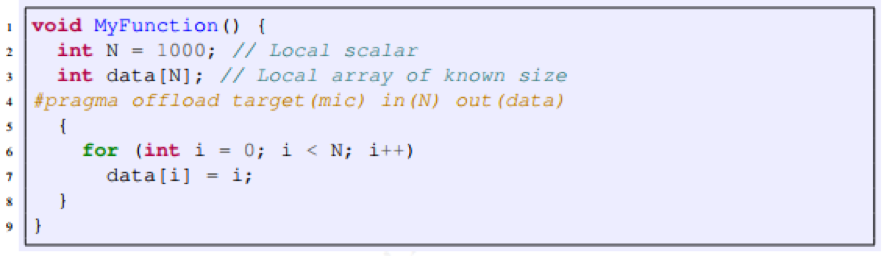
\includegraphics[scale = 0.9]{chainer11.png}
\caption{Offload of local scalars and arrays of known size using \#pragma offload.}
\end{figure}

When data is stored in an array referenced by a pointer, the array size is unknown at compile time. In this case, the programmer must indicate the array length in a clause of \#pragma offload. The length is indicated in array elements and not bytes.
\begin{figure}[H]
\centering
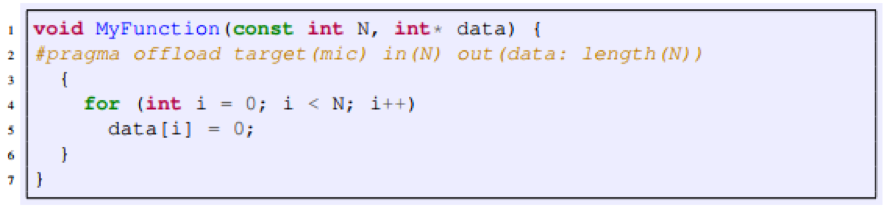
\includegraphics[scale = 0.9]{chainer12.png}
\caption{Offload of pointer based arrays of unknown size.}
\end{figure}
\subsection{Data Transfer without Computation}
If it is necessary to send data to the coprocessor without launching any processing of this data, either the body of the offloaded code can be left blank (i.e., use “{}” after pragma offload), or a special \#pragma offload\_transfer can be used.
\begin{figure}[H]
\centering
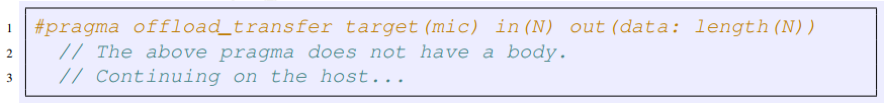
\includegraphics[scale = 0.9]{chainer13.png}
\caption{Transferring data to the coprocessor without computation.}
\end{figure}
\subsection{Data and Memory Persistence Between Offloads}
When an array is offloaded to the coprocessor, the following operations are be performed:\\
(1) Allocate a memory buffer for the array on the coprocessor.\\
(2) Copy data from host array to the buffer on the coprocessor.\\
(3) Perform offloaded calculations.\\
(4) Copy data from coprocessor buffer to the host array.\\
(5) Free the memory buffer on the coprocessor.\\
In some cases, an offload region is called multiple times with the same shape and size of some or all data structures. In this case, step (1) is necessary only in the first offload instance, and step (5) – only in the last one. 
\begin{itemize}
\item To skip the copy-in stage (2), but perform copy-out (4), use the out clause.
\item To skip the copy-out stage (4), but perform copy-in (2), use in.
\item To skip both the copy-in and copy-out, use either the nocopy clause, or in with a length of 0.
\item To preserve a memory buffer allocated on a coprocessor, clauses alloc\_if and free\_if may be used. 
\end{itemize}
\begin{figure}[H]
\centering
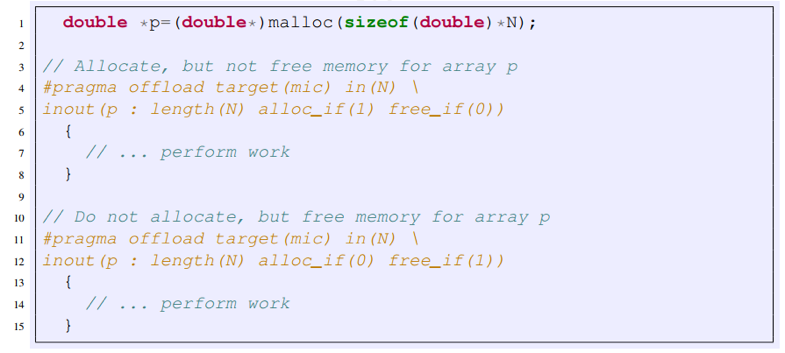
\includegraphics[scale = 0.9]{chainer14.png}
\caption{Illustration of memory buffer retention on coprocessor between offloads.}
\end{figure}
The latter data persistence instruction must always be combined with the memory-retaining clause free\_if(0) in the previous offload and alloc\_if(0) in the current offload. 
\begin{figure}[H]
\centering
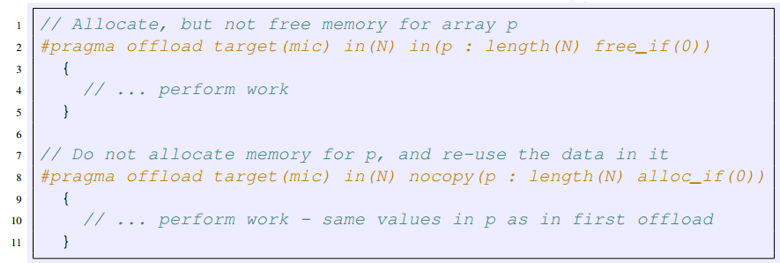
\includegraphics[scale = 0.9]{chainer15.png}
\caption{Illustration data persistence on coprocessor between offloads.}
\end{figure}

\subsection{Offloading Global and Static Variables}
When an offloaded variable is used in the global scope or with the static attribute, it must be declared with the same qualifier as an offloadable function, $\_\ _attribute\_ \_((target(mic)))$:
\begin{figure}[H]
\centering
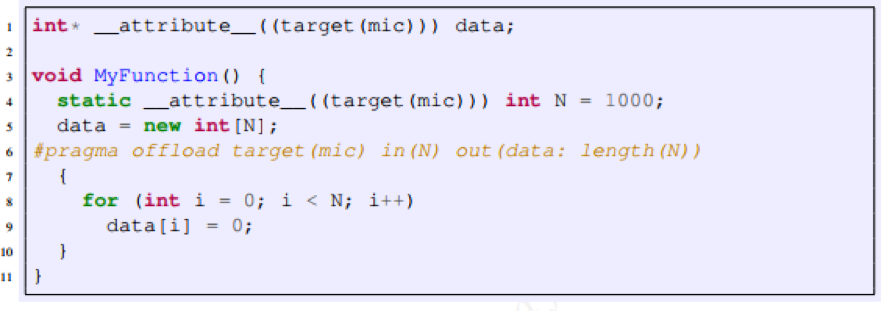
\includegraphics[scale = 0.9]{chainer16.png}
\caption{Offload of global and static variables.}
\end{figure}

\subsection{Memory retention and data persistence on coprocessor}
\begin{figure}[H]
\centering
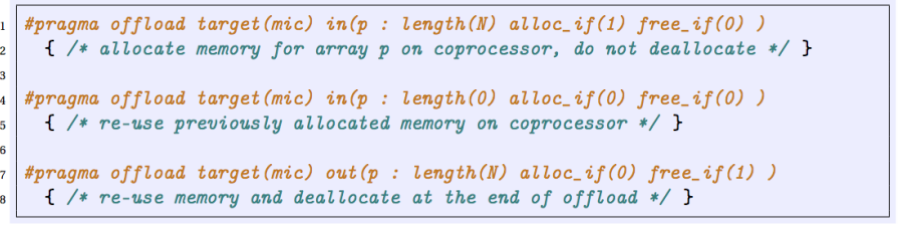
\includegraphics[scale = 0.9]{chainer17.png}
\caption{Memory retention and data persistence.}
\end{figure}
By default, memory on coprocessor is allocated before, deallocated after offload. Specifiers alloc\_if and free\_if allow to avoid allocation/deallocation. Can be combined with length(0) to avoid data transfer. Why bother: data transfer across the PCIe bus is relatively slow (6 GB/s), and memory allocation on coprocessor is even slower (0.5 GB/s).

\subsection{Asynchronous Offload}
Offload pragmas are synchronous. It is also possible to initiate asynchronous offload and data transfer in the explicit offload model. Asynchronous data transfer opens additional possibilities for optimization:
\begin{itemize}
\item Data transfer time can be masked.
\item The host processor and coprocessor can be employed simultaneously.
\item It provides a way to distribute work across multiple coprocessors.
\end{itemize}
Asynchronous data transfer is initiated by adding the specifier signal to
the offload pragma. After that, another offload pragma with the wait clause,
or \#pragma offload\_wait are used to catch the signal of the end of
the offload. 
\begin{figure}[H]
\centering
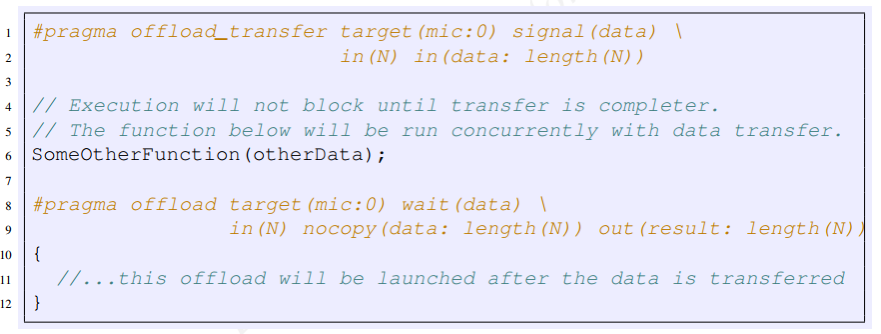
\includegraphics[scale = 0.9]{chainer18.png}
\caption{Illustration of asynchronous data transfer and wait clause.}
\end{figure}
With asynchronous offload, SomeOtherFunction() will be executed concurrently with data transport. In the second \#pragma statement, the specifier wait(data) indicates that the offloaded calculation should not start until the data transport signaled by data has been completed.

In this following code, two coprocessors are employed simultaneously using asynchronous offloads, the host code execution will wait at this pragma until the transport signaled by data has finished. This pragma is useful when it is not necessary to initiate another offload or data transfer at the synchronization point.
\begin{figure}[H]
\centering
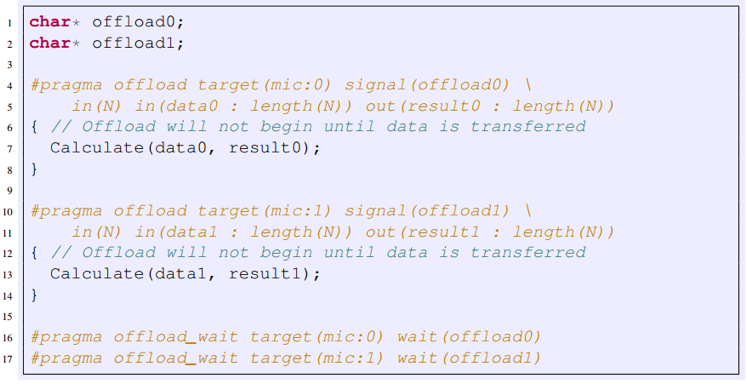
\includegraphics[scale = 0.9]{chainer19.png}
\caption{Illustration of asynchronous offload to different coprocessors.}
\end{figure}

\subsection{Target-Specific Code}
The values of tuning parameters in HPC algorithms may depend on
the amount of memory, cache size, and other parameters, which are different
between the host and the coprocessor platforms. These tuning parameters
can be multi-versioned using $ \_\_MIC\_\_$
\begin{figure}[H]
\centering
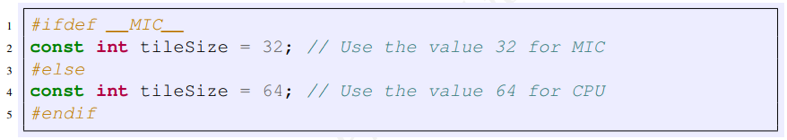
\includegraphics[scale = 0.9]{chainer20.png}
\caption{Tuning parameters can be multi-versioned using $\_\_MIC\_\_$.}
\end{figure}

\begin{figure}[H]
\centering
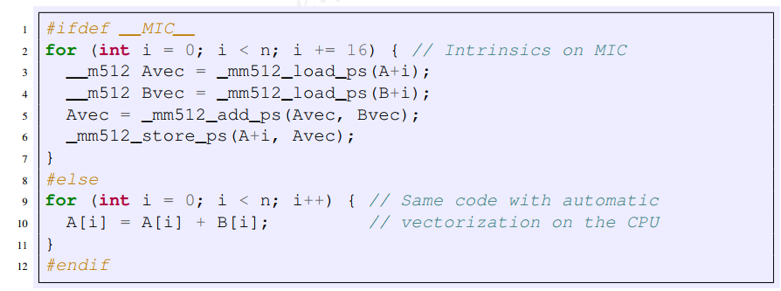
\includegraphics[scale = 0.9]{chainer21.png}
\caption{$\_\_MIC\_\_$ can protect functions unavailable on either the host, or the target platform.}
\end{figure}

\subsection{Optional and Conditional Offload, Fall-Back to Host}
If no coprocessors are found in the system, the offload code can be executed anyway, using the host processor instead of the coprocessor. This can be achieved by adding the clause optional to the offload pragma.
\begin{figure}[H]
\centering
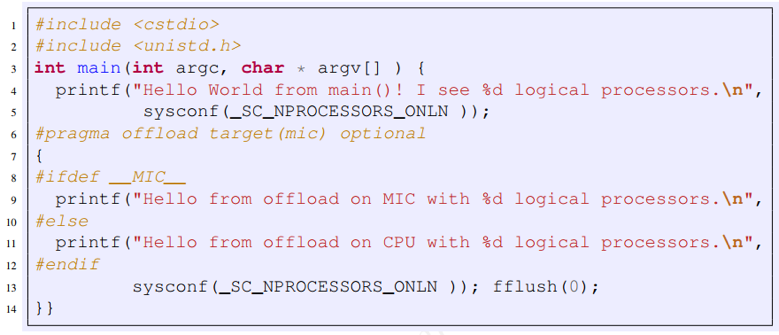
\includegraphics[scale = 0.9]{chainer22.png}
\caption{Offload-Fallback.cc: handling fall-back to host when offload fails.}
\end{figure}

This clause is if, and it takes one argument. If the argument evaluates to a non-zero value or boolean ``true", the offload will be sent to a coprocessor. If it evaluates to 0 or boolean ``false", the calculation in the scope of the offload pragma will fall back to host CPU execution.
\#pragma offload target(mic) if (N$>$1000)

Conditional offload can be used, for example, to prevent offload of a problem that is too small to pay off for the offload overhead or to distribute work between coprocessors and the CPU.

\subsection{Offload Diagnostics}
This can be generate diagnostic output for offload applications in the Linux environment variable $OFFLOAD\_REPORT$ or the function \_Offload\_report.
\begin{itemize}
\item If $OFFLOAD\_REPORT$ is unset, no diagnostic output is produced (this is
the default behavior).
\item $OFFLOAD\_REPORT$=1 prints information on the offload locations (lines
of code) and times.
\item $OFFLOAD\_REPORT$=2, in addition, produces information regarding the
amount of data traffic.
\item $OFFLOAD\_REPORT$=3 gives additional details: device initialization and
individual variable transfers.
\end{itemize}

\section{The pyMic Module}
\subsection{Introduction}
The key guiding principle of the design of the pyMIC module is to provide an easy-to-use, slim interface at the Python level. Because Numpy is a well-known package for dealing with (multi-dimensional) array data, we explicitly designed pyMIC to blend well with Numpy's ndarray class and its array operations. As we will see later, ndarrays are the granularity of buffer management and data transfer between host and coprocessors.
\begin{figure}[H]
\centering
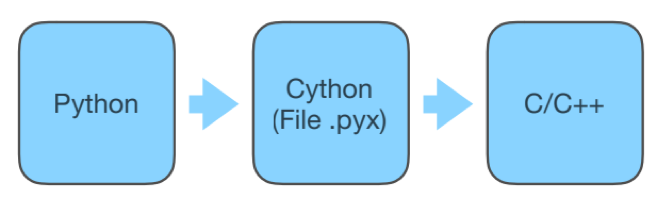
\includegraphics[scale = 0.9]{chainer23.png}
\caption{Cython Mechanism.}
\end{figure}

Several HPC applications not only use Python code, but also implement parts of their application logic in C/C++ and/or Fortran. We strive to keep pyMIC flexible, so that advanced programmers can mix Python offloads with C/C++ or Fortran offloads. For instance, one could allocate data in an ndarray, transfer it to the coprocessor through the pyMIC interface, and then use the data from an offloaded C/C++ code region in a Python C/C++ extension.
\begin{figure}[H]
\centering
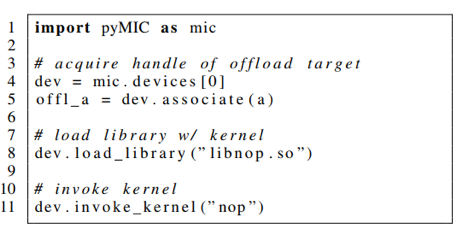
\includegraphics[scale = 0.9]{chainer24.png}
\caption{Simplistic offload example to acquire an offload device and invoke.}
\end{figure}
\begin{figure}[H]
\centering
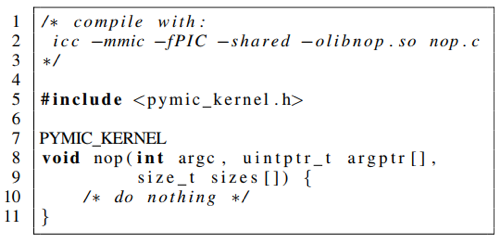
\includegraphics[scale = 0.9]{chainer25.png}
\caption{Empty kernel implementing the ``nop" kernel.}
\end{figure}

\subsection{Basic Interface}
The pyMIC interface consists of two key classes: offload\_device and offload\_array. The
offload\_device class provides the interface to interact with offload devices, whereas offload\_array implements the buffer management and primitive operations on a buffer's
data.

\begin{figure}[H]
\centering
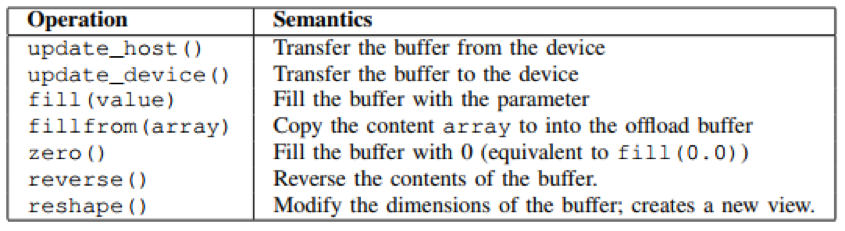
\includegraphics[scale = 0.9]{chainer26.png}
\caption{Operations of the offload array class.}
\end{figure}

\subsection{Implementation of computing function}
The layered architecture of the pyMIC module is depicted above. The top-level module contains all the high-level logic of the pyMIC module and provides the pyMIC API to be used by the application. Underneath this API module, a Python extension module (\_pyMICimpl) written in C/C++ interfaces with the offload runtime of the Intel Composer XE and its LEO pragmas. In addition, pyMIC contains a library with standard kernels that implement all the array operations of offload\_array.

\begin{figure}[H]
\centering
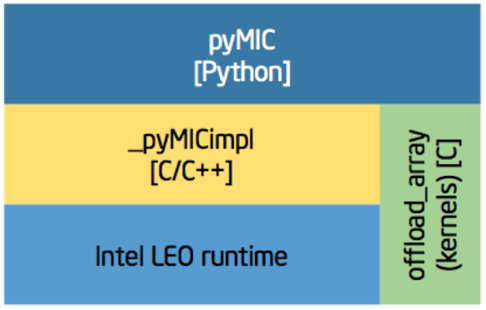
\includegraphics[scale = 0.9]{chainer27.png}
\caption{pyMIC Architecture.}
\end{figure}
We have opted to use C++ to implement the \_pyMICimpl to make use of STL for improved coding productivity. As a matter of fact, the interface of the extension is exposed to Python with the C calling convention, while the remainder of the code is plain C++. The internal code design of \_pyMICimpl provides a series of abstractions so that, for instance, the Intel LEO pragmas can easily be replaced by the HAM interface or another offload implementation.
\begin{figure}[H]
\centering
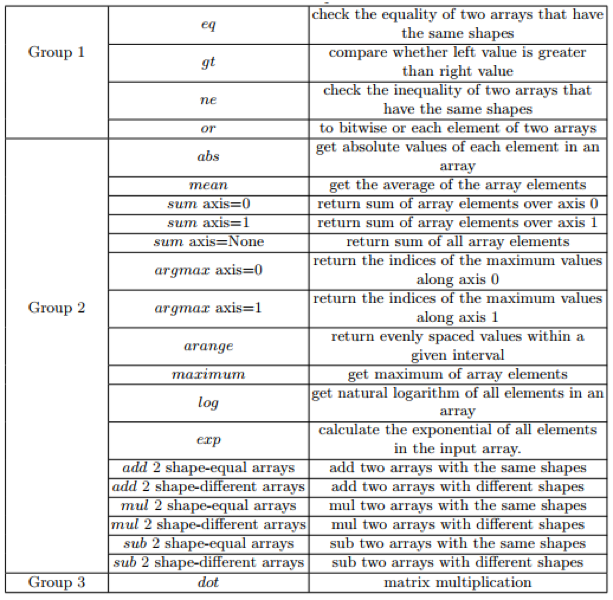
\includegraphics[scale = 0.9]{chainer28.png}
\caption{pyMIC Kernels.}
\end{figure}

\section{Experimental result with Chainer}
\subsection{Chainer}
Chainer is an open source framework designed for efficiently developing deep learning algorithms. Most existing frameworks construct a computational graph in advance of training. This approach is fairly useful, especially for implementing fixed and layer-wise neural networks like convolutional neural networks. However, with the advent of new applications and performance requirements, such as recurrent or stochastic neural networks, we need some kinds of tips to reduce the development efficiency and maintainability of the code for these complex networks. Chainer’s approach is unique for this by building the computational graph "on-the-fly" during training. It allows users to change the graph at each iteration or for each sample, which depends on conditions. This gives much greater flexibility in the implementation of complex neural networks, which leads in turning to faster iteration, and greater ability to quickly realize cutting-edge deep learning algorithms.

\begin{figure}[H]
\centering
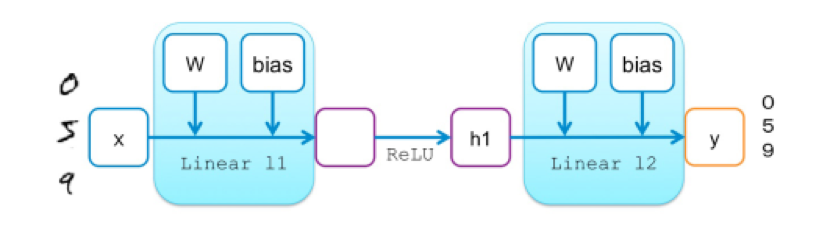
\includegraphics[scale = 0.9]{chainer29.png}
\caption{Define neural network for MINIST digit classification.}
\end{figure}

\subsection{Results}
This library is an extension of original pyMIC that is a Python offloading module for Intel coprocessor. The experimental results show that pyMIC not only outperforms compared with NumPy when considering them on two distinct hardware platforms with nearly the same theoretical peak performance, but also can be highly integrated into one popular deep learning framework Chainer with convincing performance.
\begin{figure}[H]
\centering
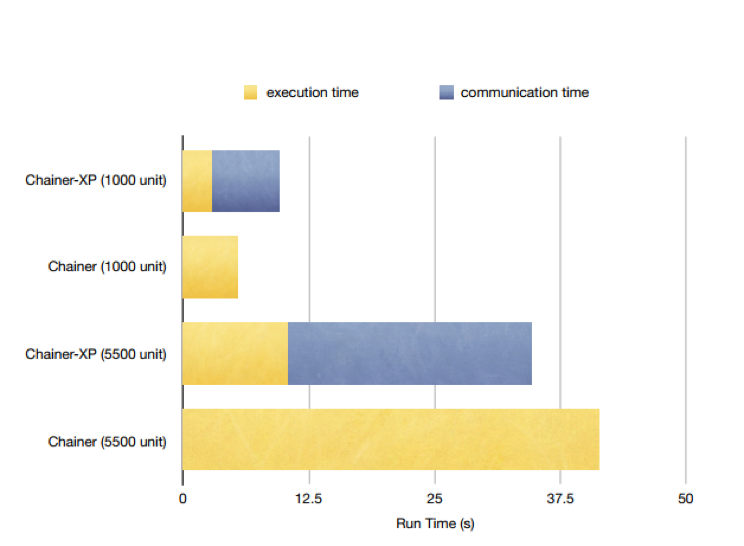
\includegraphics[scale = 0.9]{chainer30.png}
\caption{Comparing Chainer running on CPU and Xeon Phi.}
\end{figure}

\section{Reference}
\begin{itemize}
\item Klemm, M., Enkovaara, J.: \textbf{pymic: A python offload module for the intel xeon phi coprocessor}. Proceedings of PyHPC (2014)
\item Klemm, M., Witherden, F., Vincent, P.: \textbf{Using the pymic offload module in pyfr}. arXiv preprint arXiv:1607.00844 (2016)
\item Vladimirov, A., Asai, R., Karpusenko, V.: \textbf{Parallel Programming and Optimization with Intel Xeon Phi Coprocessors: Handbook on the Development and Optimization of Parallel Applications for Intel Xeon Processors and Intel Xeon Phi Coprocessors}. Colfax International (2015)
\item Backpropagation Algorithm - \url{http://deeplearning.stanford.edu/wiki/index.php/ }
\item Numpy - Broadcasting - \url{http://www.numpy.org/}
\item Cython Extension - \url{http://cython.org/}

\end{itemize}



\newpage


%\bibliographystyle{plain}
%\bibliography{refs}

\end{document}